\chapter{深層学習とロボットへの応用}
\label{chap_review}
\newpage

\section{ニューラルネットワーク}\label{sec:NeuralNetwork}
人間の脳にはニューロンと呼ばれる神経細胞が1000億個以上あり,それぞれが複数のニューロンが電気信号によって情報を伝達している.また脳にはシナプスという場所があり,ここで電気信号を細胞体へ受け渡す.細胞体はある閾値以上の電気信号がきた場合に他のニューロンへ電気信号を伝播させる(これを発火と呼ぶ).このようなニューロンとシナプスで行われる演算を模倣したアルゴリズムを作ることができれば,人間のような思考や認識をコンピュータを使って再現できると考えた.そのアルゴリズムがニューラルネットワーク(Neural Network: NN)である.

\subsection{多層パーセプトロン}
ニューラルネットワークは入力層,出力層,隠れ層から構成され,層と層の間にはニューロン同士のつながりの強さを示す重みがある.非線形問題を扱うために1986年Rumelhartによって考案されたのが,パーセプトロンを複数つなぎ合わせ入力と出力以外に隠れた層を持つ多層パーセプトロン(Multi-layer perceptron: MLP)である(\fig {mlp}).ニューラルネットワークで多層パーセプトロンの層を全結合(fully connected: FC)層とも呼ぶ.

\begin{figure}[H]
	\centering
	\begin{minipage}[b]{0.4\columnwidth}
		\centering
		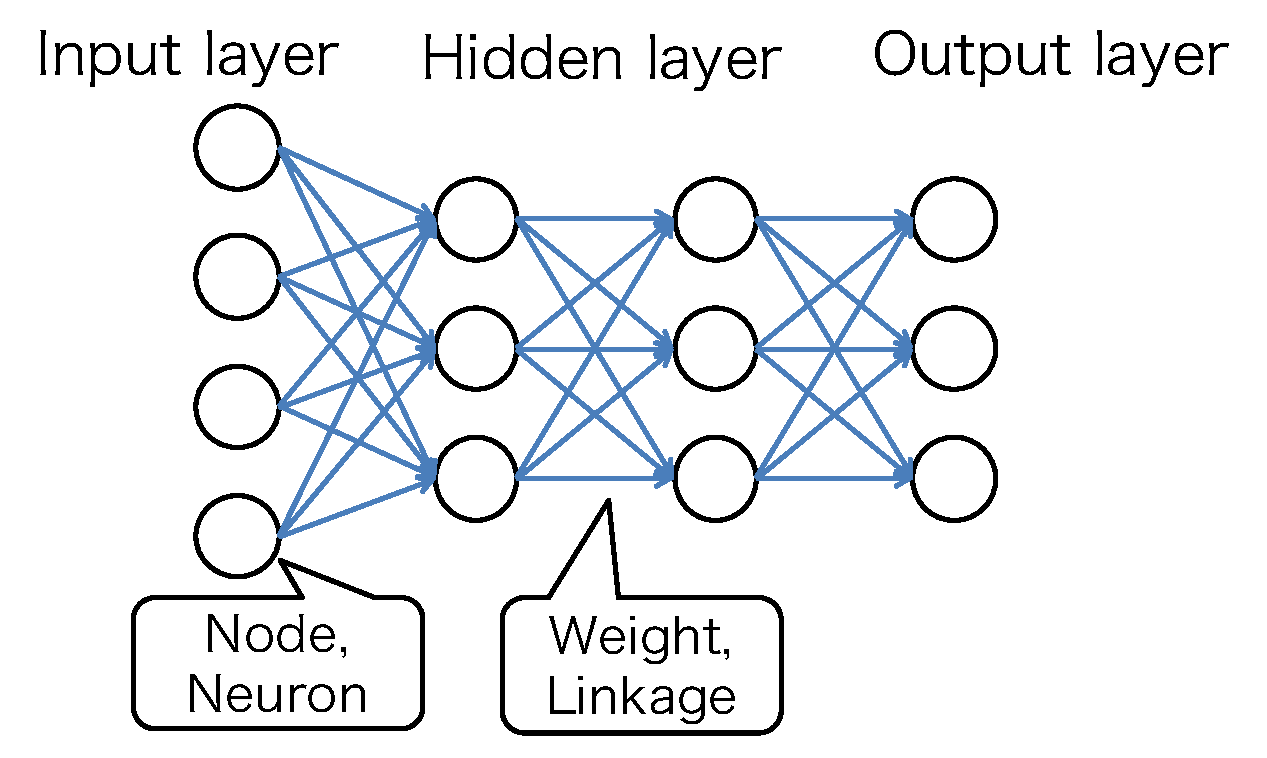
\includegraphics[width=1.2\linewidth]{figure/chapter2/MLP}
		\subcaption{Muti-layer perceptron}
		\label{fig:mlp}
	\end{minipage}
	\begin{minipage}[b]{0.4\columnwidth}
		\centering
		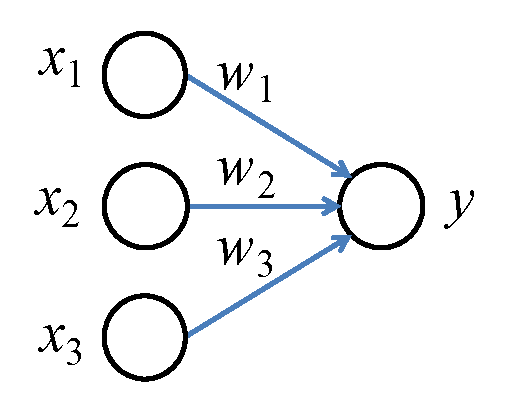
\includegraphics[width=0.7\linewidth]{figure/chapter2/simple_perceptron}
		\subcaption{Simple perceptron}
		\label{fig:perceptron}
	\end{minipage}
	\caption{Architecture of Muti-layer perceptron}
\end{figure}

\fig {mlp}における丸や矢印はそれぞれノード(またはニューロン)と重み(または結合)と呼び,ともに数値である.例えば画像を分類しようと思えば,各ピクセルの画素数を各ノードに入力する.例えば$28 \times 28$pxのグレースケール画像であれば,784個のノードが必要となる.入力データ$\bm {x}$が入力層に入ってくると,その値に重み$\bm {w}$をかけ,活性化関数$H$と呼ばれる関数に通し,結果$\bm{y}$を出力する.ここで,入力$\bm{x}$,重み$\bm{w}$,出力$\bm{y}$を太字で表したが,これらは全てテンソルであり,1つの層にあるノード$x_1, x_2, \cdots x_n$を一括して$\bm {x}$として表記している.

ここで,中間層の1つのノードについて考える.\fig {perceptron}にMLPを構成する1ユニットである単純パーセプトロンを示した.この模式図を数式で表すと次のようになる.
\begin{align}
	y & = H(\bm{w}\bm{x} + \bm{b}) \\
	& = H\left( \sum_{i=1}^3 w_i x_i + b_i \right) 
\end{align}
ここで$\bm{b}$はバイアスと呼ばれ,発火のしやすさを表している.中間層における活性化関数は,\eq {ReLU}に示す正規化線形関数(rectified linear unit: ReLU)と呼ばれる関数)がよく用いられる.
\begin{align}\label{eq:ReLU}
	H(x) = \max \left\lbrace 0, x \right\rbrace = \begin{cases}
	x & (x > 0) \\
	0 & (x \leq 0)
	\end{cases}
\end{align}
この演算を繰り返し出力層に書き出す.ここで,各層の重みの値によって出力結果は異なってくる.

出力層では,ノードの個数は区別したいクラス数分用意する.
各ノードの出力値が各クラスに属している確率を表すように,活性化関数にはソフトマックス関数を用いる(ただし二値分類の場合はシグモイド関数を用いる).ソフトマックス関数は\eq {softmax}で表される.
\begin{align}\label{eq:softmax}
	y_i = \dfrac{\exp(x_i)}{\displaystyle \sum_{k=1}^n \exp(x_k)}
\end{align}
ここで$y_i$は,出力層が全部で$n$個あるとして,$i$番目の出力であることを示す.\eq {softmax}からわかるように,入力の総和に対して1つのノードがどれくらいの値を持つかという割合で表されている.これにより各ノードの出力は確率として解釈できるため,値の一番大きいノードのインデックスを予測ラベルとして見ることができる.


\subsection{畳み込みニューラルネットワーク}
従来の画像認識では,画像から特徴を抽出しそれを識別器にかける手法が主流であった.古典的手法では画像から特徴を抽出するいわゆる特徴量設計が必要で,ここをいかにうまく設計するかがポイントであった.特徴抽出の方法として,HOG\cite{HOG}やSIFT\cite{SIFT},SURF\cite{SURF}などがあり,これらによって抽出した特徴ベクトルをSupport Vector Machine(SVM)\cite{SVM}によって識別することが多かった.

しかし,1998年にLeNetと呼ばれる畳み込みニューラルネットワーク(Convolutional Neural Network: CNN)が提案された\cite{LeNet}.CNNは畳み込み層とプーリング層からなっている.この畳み込みとプーリングの演算を通して,特徴量設計から識別までをend-to-endで行うことができる.

\begin{figure}[H]
	\centering
	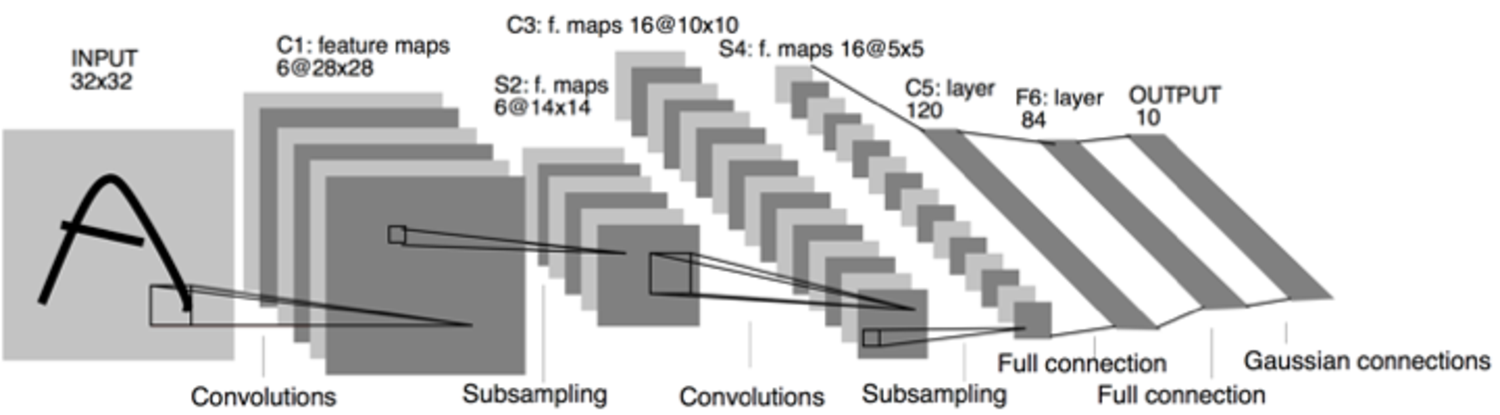
\includegraphics[width=0.7\linewidth]{figure/chapter2/LeNet}
	\caption[Architecture of convolutional neural network]{Architecture of convolutional neural network\cite{LeNet}}
	\label{fig:LeNet}
\end{figure}


%人間が物体を認識することをコンピュータにも計算させるには,画像の特徴的な部分を切り分けて数値化させる必要がある.例えば,カラー画像の場合,RGBの3色(3チャンネル)を組み合わせた画像で認識をしている.このようなフィルターの畳み込み計算を行うと,フィルターごとに異なった画像の特徴を抽出して数値化する.これが畳み込み(convolution)である.その後,画像のサイズを小さくしてコンピュータが計算コストを減らし,微小な変化に対してロバストになる仕組みしてプーリングという方法を用いる.

畳み込み層では,入力に対してフィルター(カーネルとも呼ばれる)を用意し,\eq {conv}に示す計算を行う.
\begin{align}\label{eq:conv}
	y_{i,j} & = (\bm{K} * \bm{x})_{i,j}\\
	& = \sum_m\sum_n x_{i+m, j+n} K_{m,n}
\end{align}
ここで,$\bm{K}$はフィルター,$\bm{x}$は入力,$y$は出力である.CNNではこの演算の後に活性化関数に通す.これを図で表すと\fig {conv}のようになる.

\begin{figure}[H]
	\centering
	\begin{minipage}{0.45\columnwidth}
		\centering
		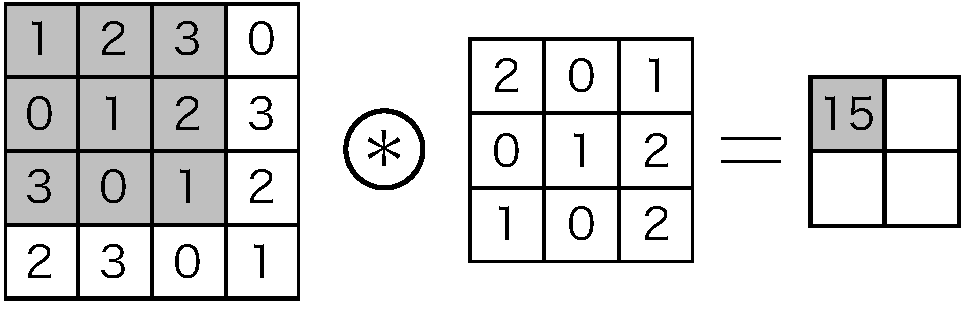
\includegraphics[width=\linewidth]{figure/chapter2/conv_ex1}
		\subcaption{}
		\label{fig:conv_ex1}
	\end{minipage}
	\hspace{10truemm}
	\begin{minipage}{0.45\columnwidth}
		\centering
		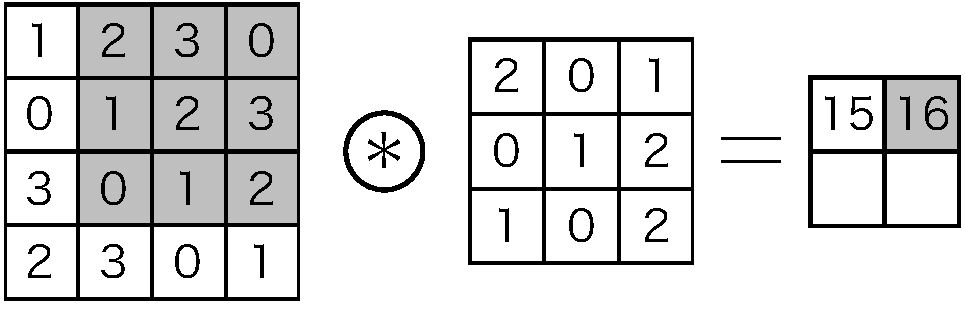
\includegraphics[width=\linewidth]{figure/chapter2/conv_ex2}
		\subcaption{}
		\label{fig:conv_ex2}
	\end{minipage}
	\begin{minipage}{0.45\columnwidth}
		\centering
		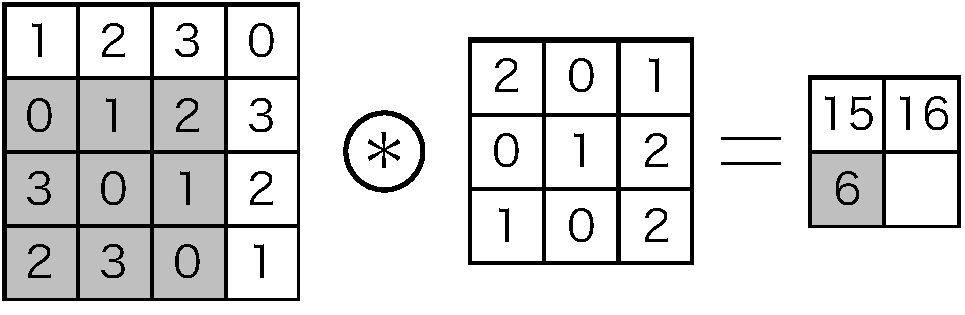
\includegraphics[width=\linewidth]{figure/chapter2/conv_ex3}
		\subcaption{}
		\label{fig:conv_ex3}
	\end{minipage}
	\hspace{10truemm}
	\begin{minipage}{0.45\columnwidth}
		\centering
		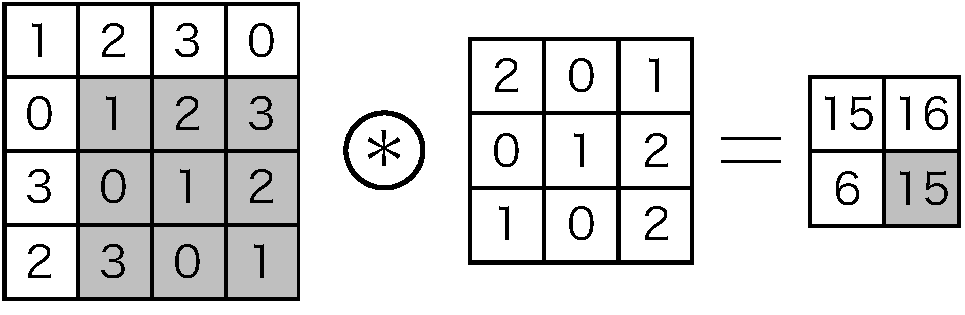
\includegraphics[width=\linewidth]{figure/chapter2/conv_ex4}
		\subcaption{}
		\label{fig:conv_ex4}
	\end{minipage}
	\caption{Operation process of convolution}
	\label{fig:conv}
\end{figure}

\fig {conv}では,フィルターのサイズは$3\times 3$であるが,大きさは任意である($3\times 3$や$5\times 5$, $7\times 7$がよく用いられる).また,フィルターは1マスずつ横にずらして計算を行っている.ずらし方をストライドといい,今回はストライド1である.CNNでは多くの場合,ストライドは1である.
このようなフィルターの畳み込み計算を行うと,フィルターごとに異なった画像の特徴を抽出して数値化することができる.

次にプーリングを行う.ここでは,画像認識で多く用いられる最大値プーリングについて述べる.\fig {maxpooling}に示すように,$2\times 2$のプールサイズを用意した時,その範囲内にある最大値を取る演算である.ストライドはプールサイズと合わせ,プーリングを行った領域と被らないようにすることが一般的である.\fig {maxpooling}ではストライド2である.

\begin{figure}[H]
	\centering
	\begin{minipage}[b]{0.4\columnwidth}
		\centering
		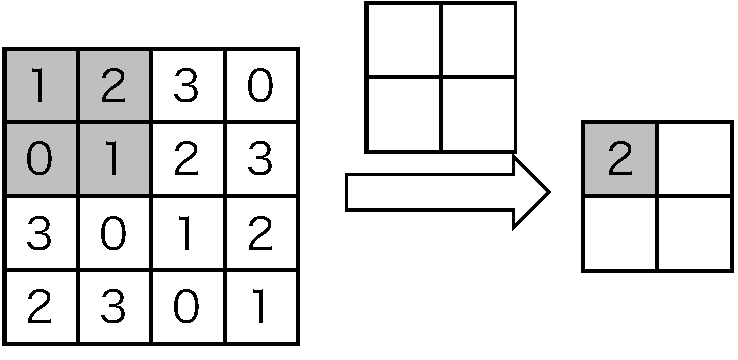
\includegraphics[width=\linewidth]{figure/chapter2/pooling_ex1}
		\subcaption{}
		\label{fig:pooling_ex1}
	\end{minipage}
	\hspace{10truemm}
	\begin{minipage}[b]{0.4\columnwidth}
		\centering
		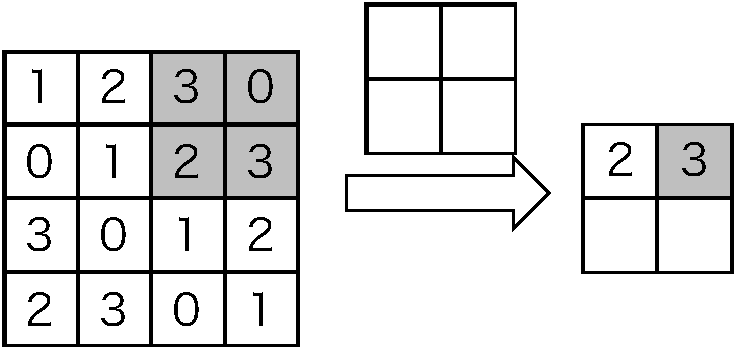
\includegraphics[width=\linewidth]{figure/chapter2/pooling_ex2}
		\subcaption{}
		\label{fig:pooling_ex2}
	\end{minipage}
	\begin{minipage}[b]{0.4\columnwidth}
		\centering
		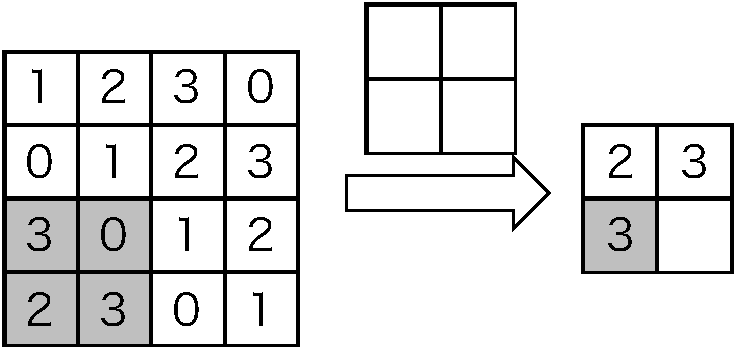
\includegraphics[width=\linewidth]{figure/chapter2/pooling_ex3}
		\subcaption{}
		\label{fig:pooling_ex3}
	\end{minipage}
	\hspace{10truemm}
	\begin{minipage}[b]{0.4\columnwidth}
		\centering
		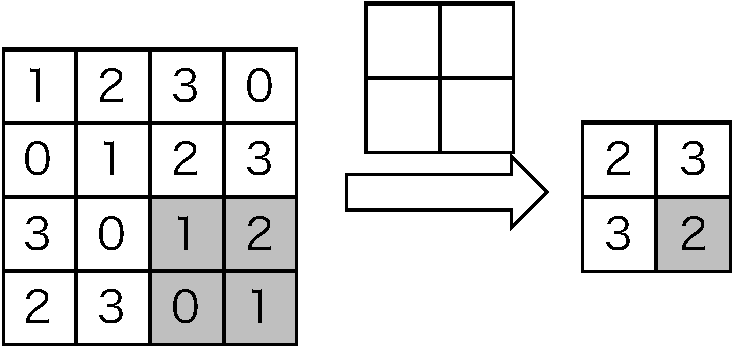
\includegraphics[width=\linewidth]{figure/chapter2/pooling_ex4}
		\subcaption{}
		\label{fig:pooling_ex4}
	\end{minipage}
	\caption{Operation process of max pooling}
	\label{fig:maxpooling}
\end{figure}

プーリング層では画像のサイズを小さくして(コンピュータの)計算コストを減らし,微小な変化に対してロバストになる.

この畳み込みとプーリングを繰り返して,入力からフィルターの数だけ特徴を抽出し,この抽出した特徴マップをFC層へ繋げて識別を行う手法がCNNである.


\section{推論と学習}
ニューラルネットワークでは推論フェーズと学習フェーズに分かれている.\ref{sec:NeuralNetwork}節は全て推論フェーズの話であり,順伝播ニューラルネットと呼ばれる.

学習フェーズでは,逆伝播ニューラルネットを用いる.逆伝播とは誤差逆伝播法(Backpropergation)\cite{Backprop}から由来している.真値からの誤差を表す損失関数(loss function)を用いて,パラメータの微分値を更新に用いる.損失関数はコスト関数,目的関数とも呼ばれる.この微分値を効率よく計算するアルゴリズムが誤差逆伝播法である.

損失関数は解く問題の目的に合わせて選ぶ必要がある.回帰問題では平均二乗和誤差(mean squared error: MSE)が用いられる.
\begin{align}\label{eq:mse}
	MSE = \dfrac{1}{N} \sum_{k}^N (y_k - t_k)^2
\end{align}
また,クラス分け問題では交差エントロピー誤差(cross entropy error)が用いられる.
\begin{align}\label{eq:crossentropy}
	CE = - \sum_k ^N t_k \ln {y_k}
\end{align}
ここで,$y$は予測ラベルで,$t$は教師ラベルである.


\subsection{最適化手法}
損失関数を用いてパラメータを更新するが,更新手法にはいくつか方法があるため,ここでは本研究で使用した最適化手法について述べる.

\subsection*{SGD}
SGDは確率的勾配降下法(Stochastic gradient descent)と呼ばれる手法で,最も単純な最適化手法である.画像認識の分野では多く使われている.

SGDでは以下の式\eq {SGD}でパラメータを更新する.
\begin{align}\label{eq:SGD}
	\bm{W} \leftarrow \bm{W} - \eta \pdif{L}{\bm{W}} 
\end{align}
ここで,$\bm{W}$は更新する重みパラメータ,$\pdif{L}{\bm{W}}$は$\bm{W}$に関する損失関数の勾配である.また$\eta$は学習率と呼ばれ,実際には0.01や0.001といった値を前もって決めて使用する.SGDはパラメータの勾配を利用して,勾配方向にパラメータを更新するステップを繰り返して,徐々に最適なパラメータへと近づける手法である.

\subsection*{Adam}
Adam\cite{Adam}はadaptive moment estimationの略で,勾配の値の1乗和と2乗和の両方をパラメータ更新に用いる手法である.以下の式\eq{adam}でパラメータを更新する.

\begin{align}\label{eq:adam}
	\bm{m} & \leftarrow \beta_1 \bm{m} + (1 - \beta_1) \pdif{L}{\bm{W}} \\
	\bm{v} & \leftarrow \beta_2 \bm{v} + (1 - \beta_2) \left( \pdif{L}{\bm{W}} \right) ^2 \\
	\bm{W} & \leftarrow \bm{W} - \eta \dfrac{\hat{\bm{m}}}{\sqrt{\hat{\bm{v}}} + \epsilon} 
\end{align}

$m_t$と$v_t$はそれぞれ、勾配の一次モーメント(平均値)と二次モーメント(分散した平方偏差)の概算値である.$\eta$,$\beta_1$,$\beta_2$はそれぞれ学習パラメータである.
また,$\hat{m}_t$,$\hat{v}_t$はそれぞれ移動指数平均を用いた際に生じるバイアス(大きさを変えてしまっていることなど)を打ち消すために正則化しており,\eq {adamhat}で表される.

\begin{align}\label{eq:adamhat}
	\hat{\bm{m}} & = \dfrac{\bm{m}}{1 - \beta_1} \\
	\hat{\bm{v}} & = \dfrac{\bm{v}}{1 - \beta_2}
\end{align}

学習パラメータはそれぞれ$\eta = 0.001$,$\beta_1 = 0.9$,$\beta_2 = 0.999$,$\epsilon = 10^{-8}$が最適だと言われている\cite{Adam}.

この損失関数のパラメータ微分を各層で行うため,並列計算を行うとバッチ処理できて高速に学習ができる.そのため並列演算を得意とするGPUを用いて学習を行う.

\subsection{過学習とその抑制}
ディープラーニングでは過学習(overfitting)と呼ばれる問題が多く起こる.過学習とは,訓練データに対してのみ適応し過ぎてしまい,訓練データに含まれないテストデータには精度が出ない状態を指す.過学習は,大量にパラメータを持つ表現力の高いモデルであることや,訓練データが少ないことなどが原因で起こる.ここでは過学習を抑制するテクニックを述べる.

\subsection*{Dropout}
Dropout\cite{Dropout}は,ネットワークのノードをランダムに消去しながら学習する手法である.訓練時に隠れ層のノードを毎回ランダムに選択し,そのノードの出力を0にする.そしてテスト時には全てのノードを活性化させ,信号を伝達させる.

Dropoutは,学習時にノードをランダムに消去することで,毎回異なるモデルを学習していると解釈でき,アンサンブル学習と同じ効果を擬似的に1つのネットワークで実現していると考えられる.アンサンブル学習とは,弱識別器を複数合わせて1つの強力な識別器とする手法で,現在でも有効な手法として用いられている.

\subsection*{Batch Normalization}
Batch Normalization\cite{BatchNorm}は,ネットワークにおける各層での活性化後の出力(アクティベーション)の分布を,適度な広がりを持つように調整する手法である.Batch Normalizationでは学習を行う際のミニバッチを単位として,ミニバッチごとに正規化を行う(\eq {BatchNorm}).
\begin{align}\label{eq:BatchNorm}
	\mu_B & = \dfrac{1}{m}\sum_{i=1}^m x_i \\
	\sigma_B^2 & = \dfrac{1}{m}\sum_{i=1}^m (x_i - \mu_B) \\
	\hat{x_i} & \leftarrow \dfrac{x_i - \mu_B}{\sqrt{\sigma_B^2 + \epsilon}}
\end{align}
ミニバッチとして$B = \{x_1, x_2, \cdots, x_m\}$という$m$個の入力データの集合に対して,平均$\mu_B$,分散$\sigma_B^2$を求め,入力データを平均0分散1となるように正規化を行う.$\epsilon$は0で除算されることを防ぐもので,極小の値を用いる.

Batch Normalizationを用いると,学習を速く進行させることができる,初期値にそれほど依存しない,過学習を抑制できるといった効果が期待できる.


\section{画像認識と深層学習}
Deep LearningとはDeep Neural Network(DNN)を指すことが多い.この"Deep"とは,ニューラルネットワークの層が深いことに由来している.

\fig {ImageNet}に画像認識タスクの精度の近年の推移を示す.これはImageNet Large Scale Visual Recognition Challenge(ILSVRC)と呼ばれる世界的な画像認識のコンペティションである(2010年から始まった).カテゴリ数は1000クラスで,画像枚数は120万枚の訓練データと15万枚のテストデータが用意されている.
\begin{figure}[H]
	\centering
	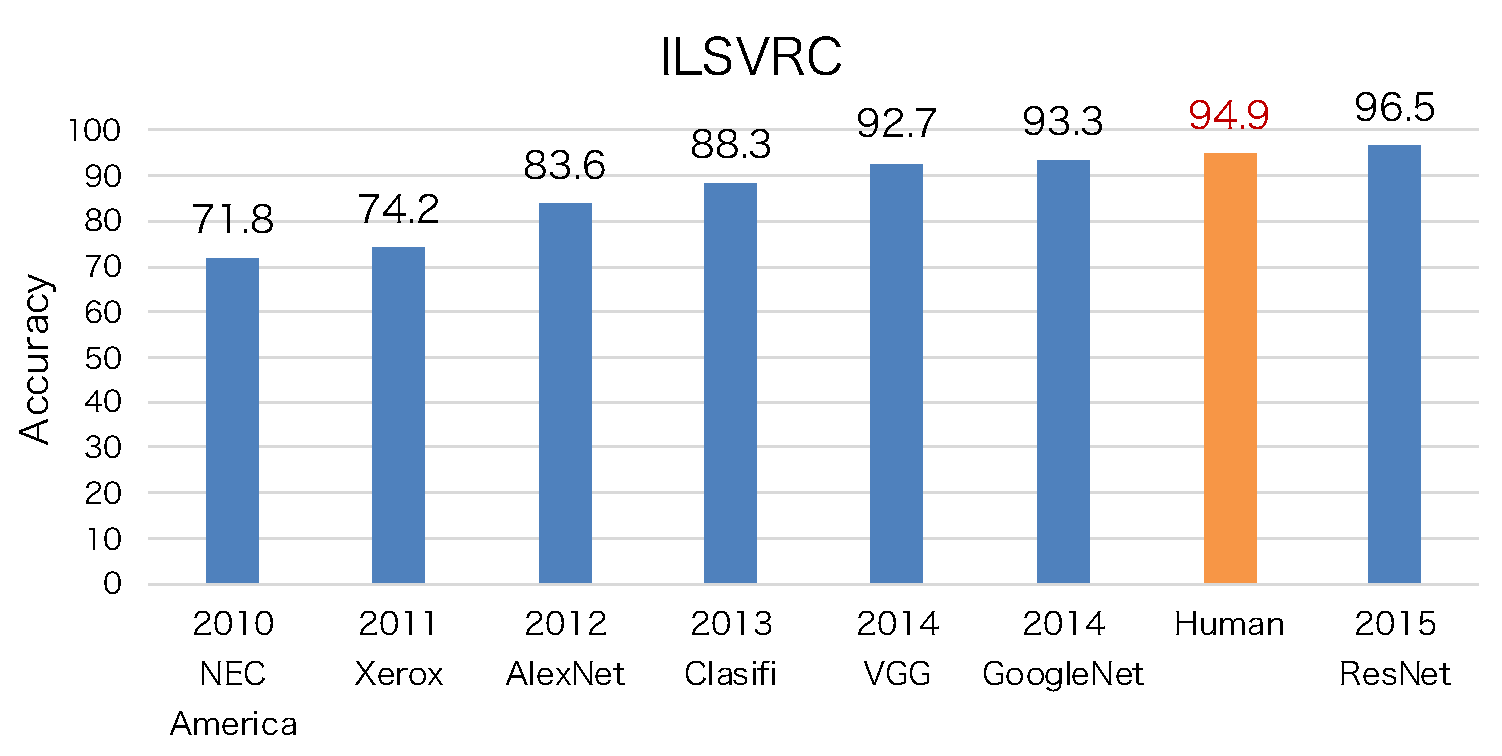
\includegraphics[width=0.7\linewidth]{figure/chapter2/ILSVRC}
	\caption{Transition of accuracy of image recognition on ILSVRC}
	\label{fig:ImageNet}
\end{figure}
2011年と2012年は約10\%もの大差でAlexNet\cite{AlexNet}が優勝している.これがディープラーニングの始まりである.AlexNetは5つの畳み込み層と3つの全結合層を持っている.2014年にはVGGNet\cite{VGGNet}やGoogLeNet\cite{GoogLeNet}が9割の精度を超えた.VGGNetはAlexNet(8層)よりさらに深い構造(19層)であり,GoogLeNetでは22層もある.そして2015年にはResNet\cite{ResNet}が人間の精度をも超える認識精度を達成した.ResNetはGoogLeNetよりもさらに深く152層もある.CNNを複数回かけて検出を行う場合,CNNの浅い層では空間分解能はあるが抽象的な情報が少なく,深い層では意味論的な情報は取得できる(ポーズ,変形など)が空間分解能が小さいため幾何学的な情報が失われるといった特徴がある.

画像処理におけるディープラーニングでは大きく3つのタスクがあり,それぞれ,クラス分類,物体検出,セグメンテーションである.ImageNetはクラス分類のタスクであったが,近年ではより難しい物体検出やセグメンテーションのタスクを含むMSCOCOというデータセットが主流になってきている.


\subsection{Classification(クラス分類)}
クラス分類は画像に写っている物体が"dog", "airplane", "bird", "toy"など事前に定義されたラベルのどれに該当するかを識別するタスクである.ILSVRCはクラス分類のコンペである.この識別は,事前に定義されたラベルの特徴べクトルと入力画像の特徴べクトルの距離計算を行い,距離値が小さければ同一,そうでなければ否と判定する.深層学習では同一人物のペア画像間の距離値が小さく,他人の画像との距離値が大きくなるような損失関数を設計しネットワークを構築することでクラス分類問題を解いている.上述したAlexNetやVGGNet,GoogLeNet,ResNetなどはクラス分類を解くためのアーキテクチャである.画像認識タスクにおいてクラス分類は後述する物体検出やセグメンテーションにおいて基幹となるタスクであるため,ResNetなどクラス分類を解くネットワーク必ずベースとして使われBackboneと呼ばれる.

ここでは,Backboneとしてよく用いられるResNetについて説明する.\fig{ResNet}にResNetのアーキテクチャを示す.
% resnetについて書く
クラス分類で使われる特徴抽出器(Feature Extraction Layer)と識別器(Classifier)に分けて解釈できる.畳み込み層で入力画像から特徴を抽出し,全結合層でクラス識別を行う.ResNet以前では特徴抽出器である畳み込み層が過学習などの問題によって深くできず,良い特徴を得られなかったためどんな識別器を用いても高い精度での識別には限界があった.しかし,ResNetで提案されたSkip connectionによって層を深くしても過学習を抑えられるようになり,劇的に改善した.Skip connectionとは\fig{skipconnection}に示すように,前の層の出力を次の層の出力と足し合わせる結合である.例えば前の層が良い特徴であって,次の畳み込みによって失われてしまっても,Skip connectionによって良い特徴を保ったまま次の層へ進めることができるようになる.言い換えるとSkipされた層が有用であるかどうかを自動で判断できるようになる.

\begin{figure}
    \centering
    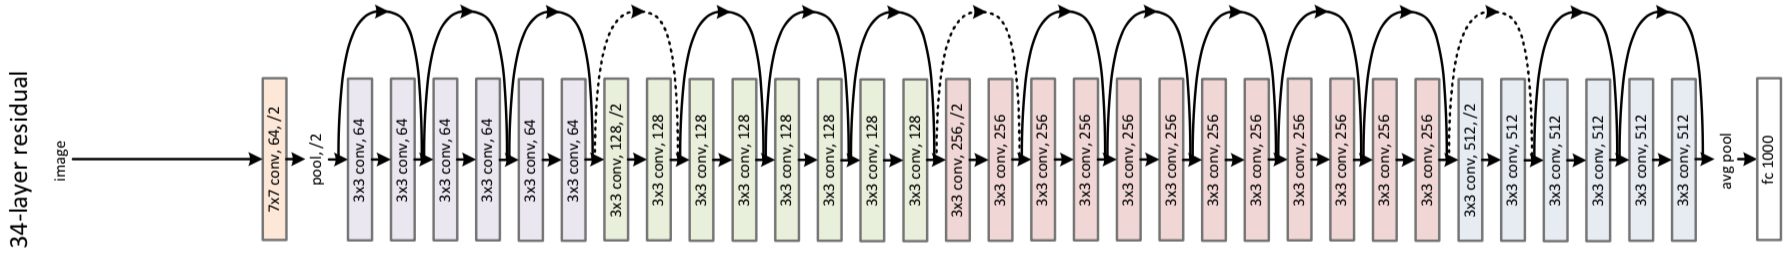
\includegraphics[width=\linewidth]{figure/chapter2/resnet34}
    \caption{Architecture of ResNet34.}
    \label{fig:ResNet}
\end{figure}

\begin{figure}
    \centering
    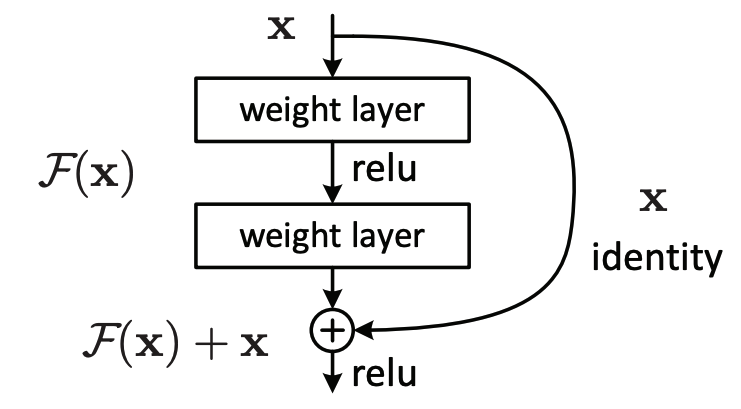
\includegraphics[width=0.5\linewidth]{figure/chapter2/skipconnection}
    \caption{Residual block: Skip Connection}
    \label{fig:skipconnection}
\end{figure}



\subsection{Object Detection(物体検出)}
物体検出とはBounding Boxで物体の位置とその物体の種類を特定する方法である.物体検出で主流であるのはFaster R-CNNである\cite{fasterRCNN}.\fig{fasterRCNN}に示すように,Faster R-CNNでは特徴抽出器であるCNNとRegion Proposal Network(RPN)の2つからなる.CNNで得た特徴マップの各点を中心としたBounding Box(BBox)を,1辺の長さおよび縦横比を変えて複数用意しRPNに入力する.RPNでは入力されたBBoxに物体か背景かを判定し,物体ならばGround truthからどれだけずれているかを学習する.これにより入力画像内のどこに物体がいるかという物体候補領域(Region of Interest: RoI)を決定する.CNNによって抽出した特徴マップと求めたRoIを照らし合わせ,該当する特徴マップをプーリングして物体候補ごとの固定サイズの特徴マップを作る(RoI pooling).RoI poolingされた特徴マップから識別器によってどのクラスに属するのか決定する.
以上のようにして,Faster R-CNNではモデル全体をEnd-to-Endで学習できる.

\begin{figure}[H]
    \centering
    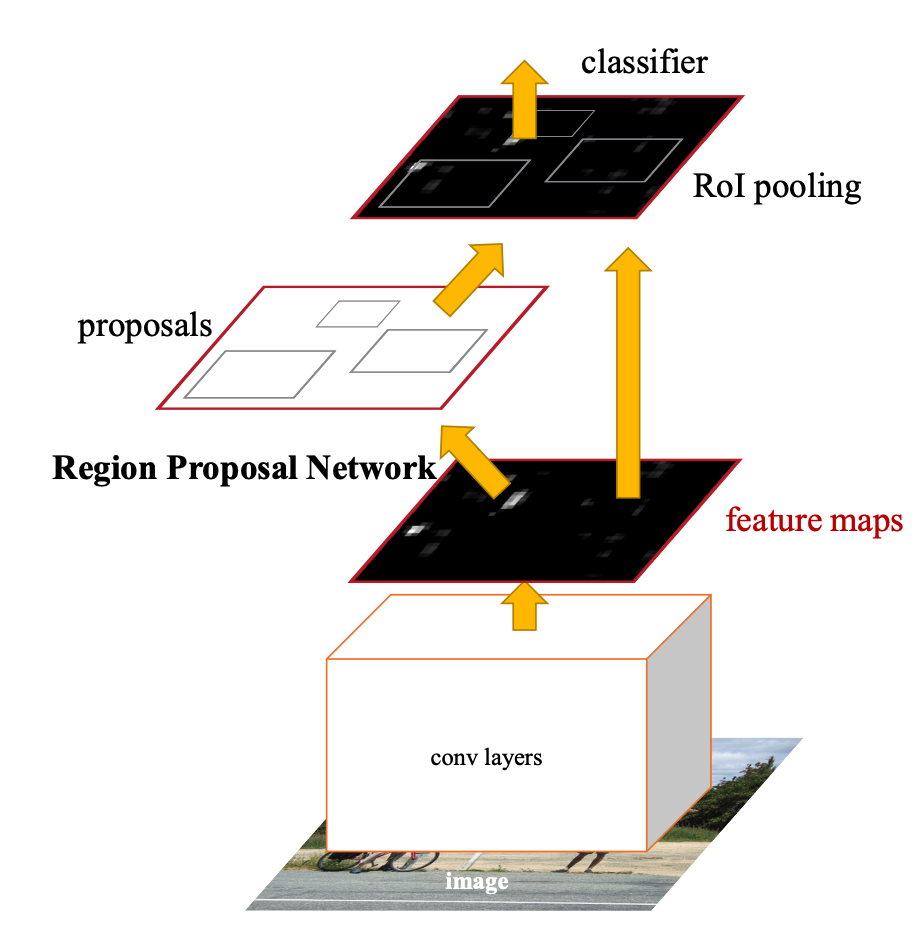
\includegraphics[width=0.7\linewidth]{figure/chapter2/fasterr-cnn}
    \caption[Architecture of Faster R-CNN.]{Architecture of Faster R-CNN\cite{fasterRCNN}.}
    \label{fig:fasterRCNN}
\end{figure}


\subsection{Segmentation(セグメンテーション)}
セグメンテーションにはSemantic Segmentation(セマンティックセグメンテーション)とInstance Segmentation(インスタンスセグメンテーション)の2つがある.

セマンティックセグメンテーションとは画像をピクセルレベルで認識することである.画像内の各画素をオブジェクトクラスに割り当てる手法である.

セマンティックセグメンテーションにおいて最初にCNNを使った手法はFully Convolutional Network(FCN)である\cite{FCN}.これはクラス分類に使われるネットワークの全結合層を畳み込み層に置き換えて,最終出力を2次元マップにするネットワークである(\fig{FCN概要}).\fig{FCN最終層}のように,これによりピクセル単位でクラス分類の結果がヒートマップとして出力される.

特徴マップのサイズはMax Poolingを経て小さくなっているため,入力画像に対して特徴マップのサイズは小さくなっている.そのためこれをUp samplingして入力画像のサイズまで拡大する.Up samplingには逆畳み込み(Deconvolution)を行う.逆畳み込みとは畳み込みの逆操作によって特徴マップから畳み込む前の画像・特徴を復元するのではなく,元となる特徴マップをpaddingやdiliateによって拡大してから畳み込む操作である.数学的にはカーネルの転置で畳み込むため転置畳み込み(Transposed Convolution)とも呼ばれる.またFCNでは途中の畳み込み層の出力も使いPoolingによって失われた細かい位置情報も利用しており,これによって出力画像がぼやけずに物体の詳細な情報を捉えたセグメンテーションが可能となる.

\begin{figure}[H]
    \centering
    \begin{minipage}[t]{0.45\columnwidth}
        \centering
        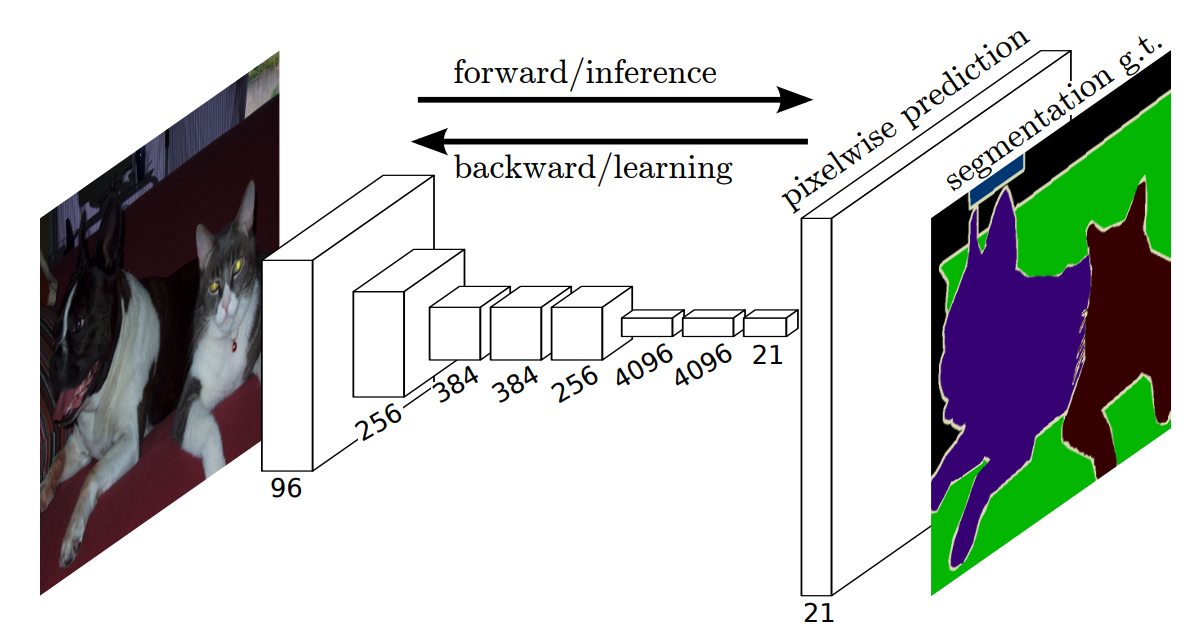
\includegraphics[width=\linewidth]{figure/chapter2/FCN_architecture}
        \subcaption[FCN framework.]{FCN framework\cite{FCN}.}
        \label{fig:FCNアーキテクチャ}
    \end{minipage}
    \begin{minipage}[t]{0.05\columnwidth}
        \hspace{5pt}
    \end{minipage}
    \begin{minipage}[t]{0.45\columnwidth}
        \centering
        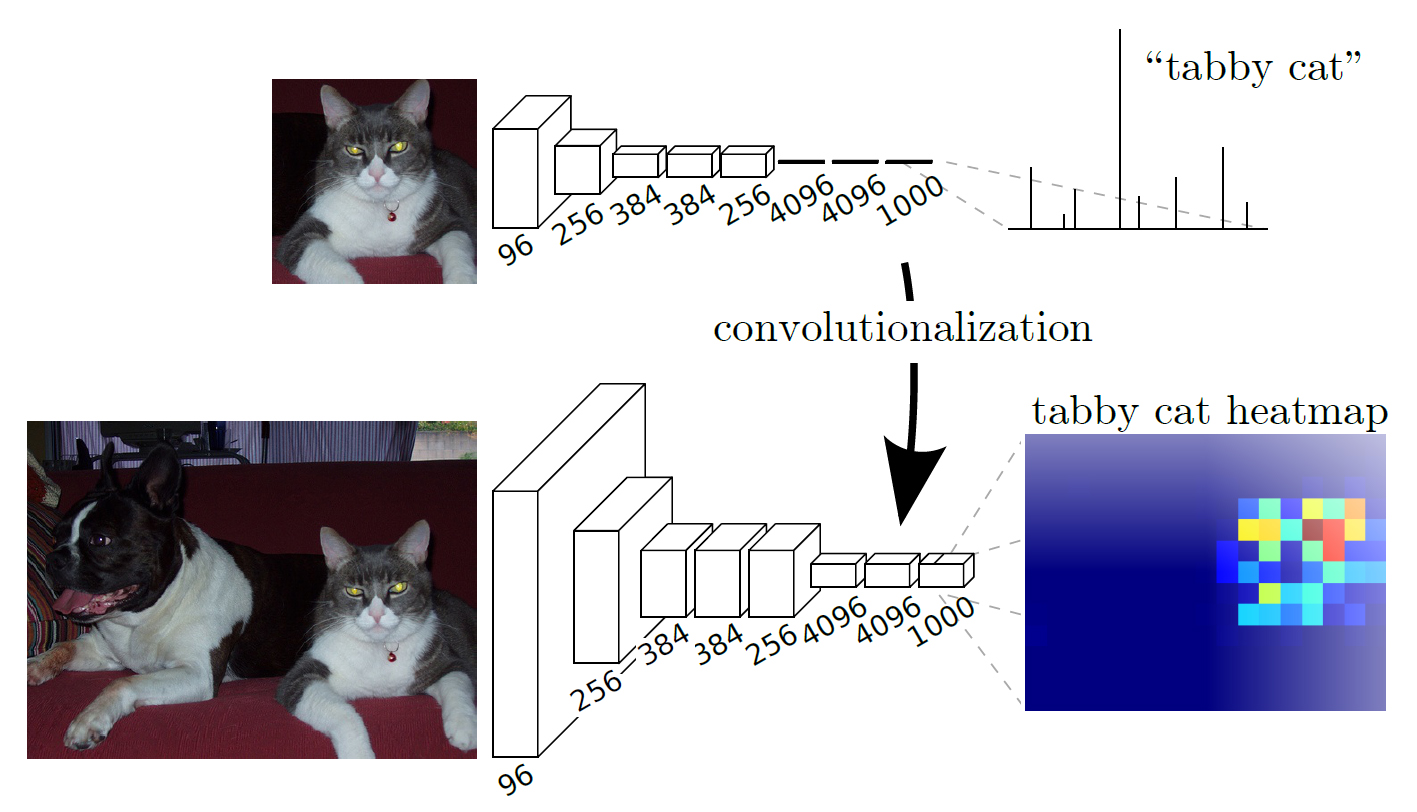
\includegraphics[width=\linewidth]{figure/chapter2/FCN_output_heatmap}
        \subcaption[Transforming fully connected layers into convolution layers.]{Transforming fully connected layers into convolution layers\cite{FCN}.}
        \label{fig:FCN最終層}
    \end{minipage}
    \caption{Architecture of FCN.}
    \label{fig:FCN概要}
\end{figure}


インスタンスセグメンテーションとは同じクラスの物体も別として認識することである.まず入力画像に対して物体検出を行い,検出したBBox内でセグメンテーションを行う.すなわち,インスタンスセグメンテーションは物体検出とセマンティックセグメンテーションのハイブリッドと言える.インスタンスセグメンテーションでよく使われる手法はMask R-CNNである\cite{MaskRCNN}.

Mask R-CNNはFaster R-CNNをベースとしたアーキテクチャで,RPマップでDetection \& Classification branchとSegmentation branchに分岐する.Detection \& Classification branchはFaster R-CNNとほぼ同様であるため説明は割愛する.Segmentation branchではFPN\cite{FPN}と同じ構造であり,畳み込みを複数回行い最後に逆畳み込みを処理することで提案候補領域におけるマスクを生成する.

\begin{figure}[H]
    \centering
    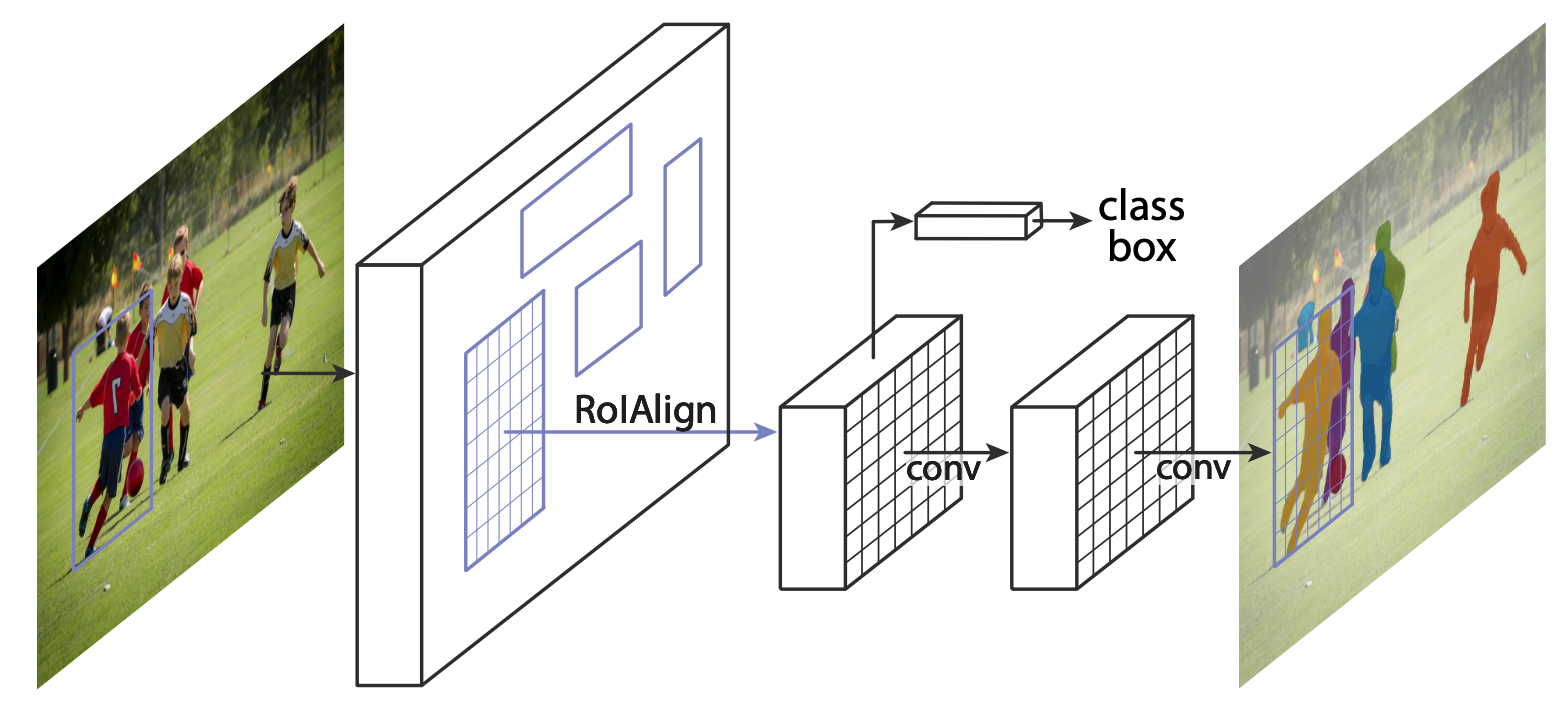
\includegraphics[width=0.7\linewidth]{figure/chapter2/mrcnn}
    \caption[Architecture of Mask R-CNN.]{Architecture of Mask R-CNN\cite{MaskRCNN}.}
    \label{fig:mrcnn}
\end{figure}



\subsection{画像認識における評価指標}
機械学習における評価指標を説明する上で混同行列というものを用いる.\tab{混同行列}に2クラス分類における混同行列を示す.混同行列の要素はTrueは正解でFalseは不正解を示しており,Positiveは予測が真,Negativeは予測が偽を出力することを表している.すなわち,$TP$は正解ラベルを正しく予測できた,$TN$は正解ラベルじゃないものを正解じゃないと予測できたことを示しており,一方$FP$は正解じゃないものを正解と予測してしまった,$FN$は正解ラベルを正解と予測できなかったことを示している.この混同行列の要素を用いて,\eq{精度}に示す3つの評価指標を定義する.

\begin{table}
    \centering
    \caption{Confusion Matrix on 2 class classification.}
    \begin{tabular}{|c|c|c|c|}\hline
        \multicolumn{2}{|c|}{} & \multicolumn{2}{c|}{Actual} \\ \cline{3-4}        \multicolumn{2}{|c|}{} & Positive & Negative \\ \hline
        \multirow{2}{*}{Predicted} & Positive & True Positive($TP$) & False Positive($FP$) \\ \cline{2-4}
        & Negative & False Negative($FN$) & True Negative($TN$) \\ \hline
    \end{tabular} 
    \label{tab:混同行列}
\end{table}

\begin{align}\label{eq:精度}
    \mathrm{Accuracy} & = \frac{TP+TN}{TP+FP+TN+FN} \notag \\ 
    \mathrm{Precision} & = \frac{TP}{TP+FP} \\
    \mathrm{Recall} & = \frac{TP}{TP+FN} \notag
\end{align}
Accuracyは正解率と呼ばれ,モデルの予測結果全体と答えがどれだけ一致しているか示す割合である.一般にモデルの精度というとAccuracyを指す事が多い.
Precisionは適合率と呼ばれ,モデルが真と予測結果全体の中で実際に正解である割合である.つまり誤検知にどれだけ強いかを示す.
Recallは再現率と呼ばれ,モデルの予測で出力されるもののうち実際に正解である割合である.つまり,見逃しにどれだけ強いかを示す.

他クラス分類では各クラスのPrecisionやRecallをクラス数で平均してAverage Precision(AP)やAverage Recall(AR)とする.

一方,物体検出やセグメンテーションにおける評価指数としてはIoU(Intersection over Union)を使う.\fig{IoU}に示すように,IoUは予測結果と教師ラベルがどれだけ重なっているかを表す.数式では混同行列の要素を使って
\begin{align}\label{eq:IoU}
    \mathrm{IoU} = \frac{TP}{TP+FP+FN}
\end{align}
と表す.
\begin{figure}[H]
    \centering
    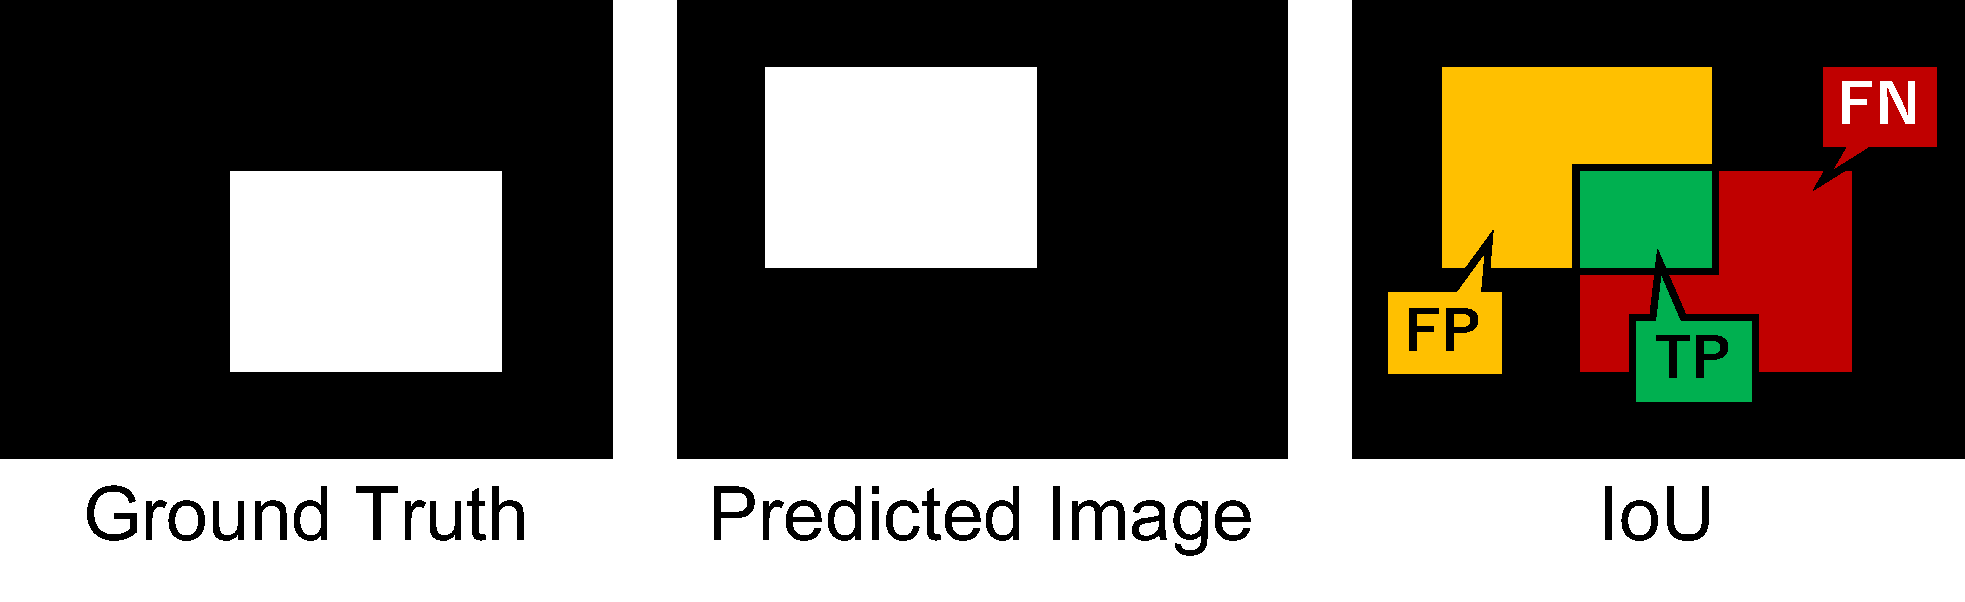
\includegraphics[width=\linewidth]{figure/chapter2/IoU}
    \caption{Example image of IoU.}
    \label{fig:IoU}
\end{figure}

また,物体検出やセグメンテーションではpixel-wiseで予測結果が出力されるため,APやARをさらに画素全体で平均を取ってmean Avereage Precision(mAP)やmean Average Recall(mAR)とする.

なお,MSCOCOと呼ばれるデータセット\cite{COCO}ではCOCO AP,COCO ARと呼ばれる独自の評価指標を用いている.\fig{COCOAP}にCOCOの評価指標のまとめを示す.
mAPやAPの決め方はひとつでなく,IoUの閾値によってそれを物体と認めるか背景とするかによって変わってくる.COCOのmAPは101pointの補間APであり,COCOでは複数のIoUを基準とするmAPを導出し,それを平均したものをAPとしたものも採用している.$\mathrm{IoU} = 0.50:0.95$は0.05刻みに0.50--0.95まで基準IoUを変えたmAPの平均である.
COCO ARは画像ごとの検出数(maxDets)を1,10,100のいずれかに固定した時のRecallを測定する.
また,AP,ARともにsmall \/ medium \/ largeに分けたオブジェクトの大きさ(Area)ごとの値も測定している.

\begin{figure}[H]
    \centering
    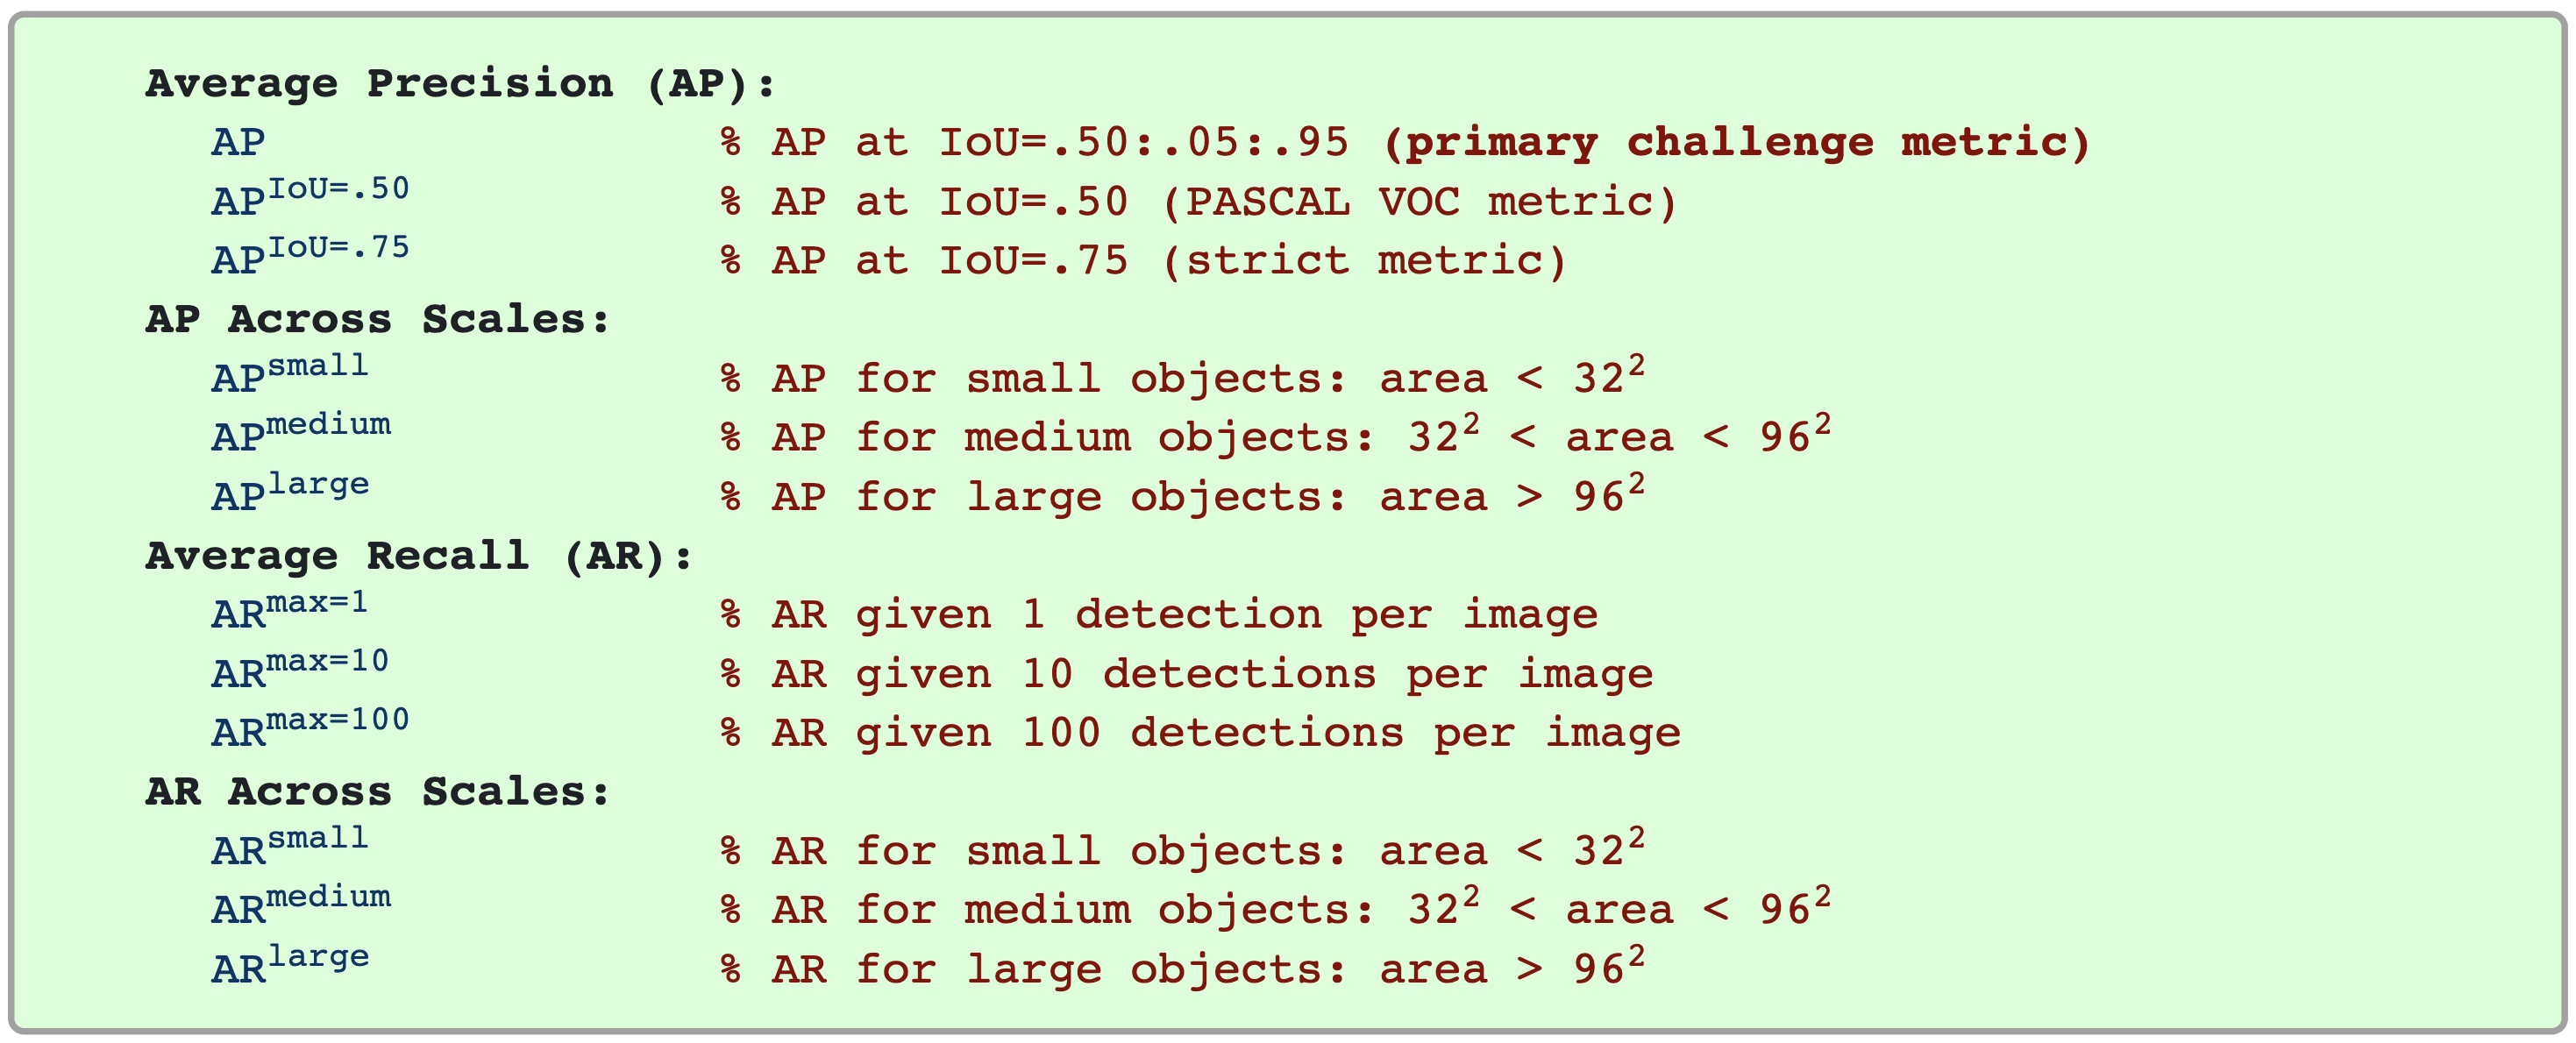
\includegraphics[width=\linewidth]{figure/chapter2/cocoAP}
    \caption[Other metrics collected for the COCO dataset.]{Other metrics collected for the COCO dataset\cite{COCO}}
    \label{fig:COCOAP}
\end{figure}

他にもいくつか細かい指標があるが,本研究では\fig{COCOAP}に示す$AP$と$AR^{max=100}$を使用した.

\section{強化学習}\label{sec:強化学習}
% 上の話は教師あり学習で,ここからは強化学習という分野である.
今まで述べてきたことは全て教師あり学習と呼ばれる手法であり,機械学習の1種である.ここからは強化学習という機械学習について述べる.

\subsection{マルコフ決定過程}
\fig {RLframework}に強化学習の概念図を示す.強化学習は,エージェントと呼ばれるプレーヤーが,与えられた環境と相互作用し,探索と知識の利用を行って目標を達成する方法を求める.強化学習は教師あり学習に似ているが,教師による明確な「答え」は提示されない.代わりに「行動の選択肢」と「報酬」が提示される.ここで,強化学習においての報酬は「各行動」に対してではなく,「連続した行動の結果」に対して与えられる.この報酬を最大化することが強化学習の目的である.
\begin{figure}
    \centering
    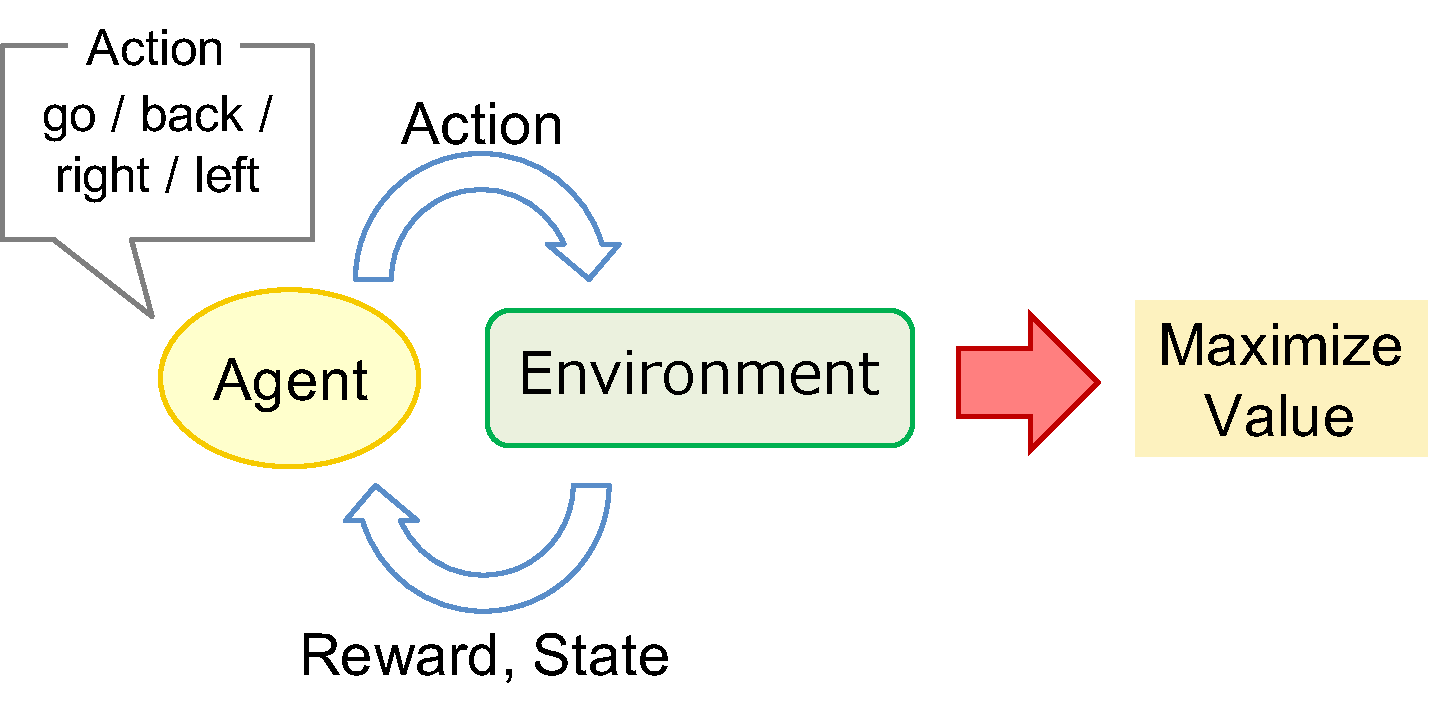
\includegraphics[width=0.7\linewidth]{figure/chapter2/RL_framework}
    \caption{Framework of Reinforcement learning}
    \label{fig:RLframework}
\end{figure}
この\fig {RLframework}を表す数理モデルとして,マルコフ決定過程(Markov Decision Process: MDP)がある.MDPは時刻$t$における状態を$s_t$,行動を$a_t$,報酬を$r_t$,状態$s_t$における行動を返す方策$\pi(a_t|s_t)$,次の状態$s_{t+1}$へ移る状態遷移確率$P(s_{t+1}|s_t, a_t)$によって記述される確率過程である.マルコフというのはマルコフ性という意味で,次の行動$s_{t+1}$には現在の状態$s_t$しか関与しないという性質を表している.1回の報酬を指標にに最適な行動を求めてはすぐに局所解に落ち着いてしまい,後に来る大きな報酬を得ることができないため,よい指標にはならない.そこで,ある期間で得られた累積の報酬(収益)$R_t$を導入する.
\begin{align}\label{eq:reward}
    R_t & = \sum _{\tau=0} ^{\infty} \gamma ^\tau r_{t+1+\tau} \\
        & = r_{t+1} + \gamma r_{t+2} + \gamma ^2 r_{t+3} + \cdots
\end{align}
と表され,これを割引報酬和(discounted total reward)と呼ぶ.ここで$\gamma(0<\gamma<1)$は割引率と呼び,未来の報酬をどの程度割り引くかを決めている.概ね1に近い値を用いる.この収益は,機関の中で報酬の和を取るため,ある行動が期間内における報酬の獲得に結び付いていた場合には,それがずっと後のことであっても,指標に反映することができる.

しかし収益は,区間の開始時点での状態に依存して,相互作用の内容が確率的に決定されるため,収益も確率的に変動してしまう.そのため,状態$s$と行動$a$を条件として収益の期待値を取り,これを行動価値(action value)と呼ぶ.行動価値関数$Q(s,a)$は,ある状態から方策$\pi$に従って行動を決定したときに得られる収益の期待値であるから,

\begin{align}\label{eq:Qfunction}
  Q^{\pi}(s_t, a_t) & = \mathbb{E}\bigl[ \bigl. R_{t+1} \bigr| s_t, a_t\bigr] \\
    & = \underset{s_{t+1}, a_{t+1} }{\mathbb{E}}\bigl[ \bigl. r_t + \gamma Q^{\pi}(s_{t+1}, a_{t+1}) \bigr| s_t, a_t \bigr]
\end{align}
で表される.これを指標として,最適な方策$\pi ^*$に基づく最適行動価値関数$Q^*$を求める.

最適価値関数を求める方法として,Temporal-Difference Learning(TD学習)が用いられる.TD学習は,環境のモデルを使わず経験的に学習を行い,最終結果を待たずに評価を途中で更新する.TD学習は次のステップを待ち価値関数を更新する.
\begin{align}\label{eq:TD}
Q(s_t, a_t) \leftarrow & Q(s_t, a_t) + \alpha (r_{t+1} + \gamma Q(s_{t+1}, a_{t+1}) - Q(s_t, a_t) )
\end{align}
$\alpha(0<\alpha<1)$は学習率である.ここで,$r_{t+1} + \gamma Q(s_{t+1}, a_{t+1}) - Q(s_t, a_t)$をTD誤差と呼び,収束からの離れ具合を示す.学習が収束したとすればTD誤差が0になり,その収束値が最適価値関数となる.

\subsection{Q-Learning}
Q学習\cite{QLearning}と呼ばれる手法ではTD誤差に基づいて,次のように価値関数$Q$を更新する.
\begin{align}\label{eq:Qupdate}
    Q(s,a) \leftarrow & Q(s,a) + \alpha (r + \gamma\underset{a'}{\max}{Q(s',a')} - Q(s,a))
\end{align}
更新式で実際に採用した行動$a'$を使っていない(方策に関わらず価値関数の最大値を与える行動を使っている)ことが特徴である.ここで,方策$\pi$としては,まずはランダムに行動することで状態と行動のセット$(s,a)$を蓄積していき,その中で行動価値関数が最大となるような行動を取る.これを$\epsilon$-greedy方策と呼ぶ.確率$\epsilon$でランダムに行動することで,局所解に陥らずに最大値へ収束することができる.

端的に言えば,「どの状態で、どう行動したら、どういう報酬が得られるのか」を明らかすることがQ-Learningである.実際はこの報酬の見込みの表形式で表し,これをQ-Tableと呼ぶ.

Q-LearningはQ-Tableが求まれば良いが,環境から得られる状態の次元や行動の次元が大きいと求められない場合がある.そのため,Q-Learningを設計する場合は,環境から特徴を取り出し低次元にする必要がある.また,行動も連続的な行動ではなく,離散的な行動選択に絞る必要がある.


\section{機械学習のロボット制御への応用}
強化学習は戦略が必要なタスクに適用できる.ロボット制御への応用も多く研究されている.例えばロボットによるピッキングタスクを行うとすると,多くのパラメータを制御する必要があり使用する環境ごとにチューニングする必要があるが,強化学習を用いることで最適な行動をするようにパラメータを獲得でき,かつどんな環境に対してもロバストになる.ここではどのように強化学習を適用するか,先行研究を追いながら説明する.

Guらは人間の手を介さずドアを開ける動作を初めて成功させた\cite{Gu2017}(\fig {Gu}).ここでは,Q-LearningをベースとしたNormalized Advantage Function(NAF)という手法\cite{NAF}を用いている.観測する状態として,7つの間接角度とその時間微分,ハンドエフェクタ・手・ドアのそれぞれの位置,手・ドアのそれぞれの角度の計25次元を入力し,Actionは連続値で出力する.シミュレーション上で4機で非同期分散学習させた後,実世界では最大2機で非同期分散学習を行った.実世界では成功率100\%になるまでに1機では4時間,2機では2.5時間という短い時間で達成した.シミュレーションから実世界への転移は難しいことが多く,Guらは成功判定を緩めることで解決した.
\begin{figure}
    \centering
    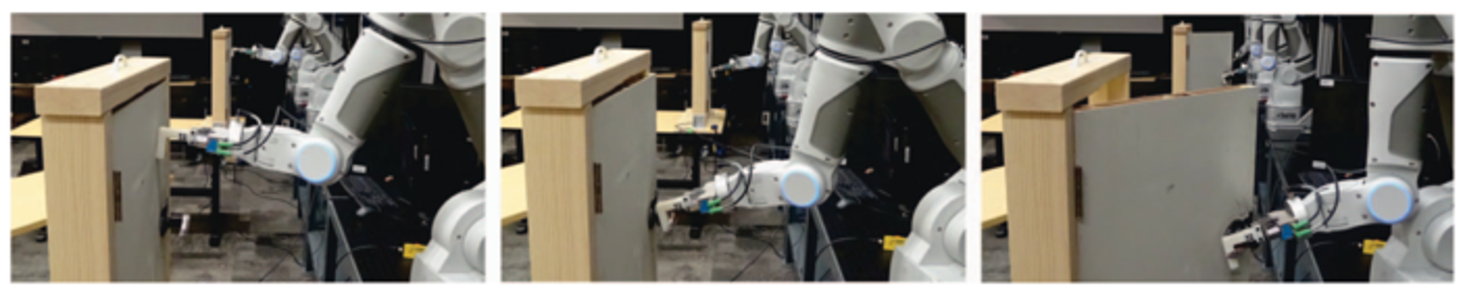
\includegraphics[width=\linewidth]{figure/chapter2/Gu}
    \caption[Two robots learning to open doors using asynchronous NAF. The final policy learned with two workers could achieve a 100\% success rate on the task across 20 consecutive trials.]{Two robots learning to open doors using asynchronous NAF. The final policy learned with two workers could achieve a 100\% success rate on the task across 20 consecutive trials\cite{Gu2017}.}
    \label{fig:Gu}
\end{figure}

またDmitryらは,Q-Learningを改良したQT-optという手法を提案した\cite{Dmitry2018}(\fig {Dmitry}).これはより汎用性の高いタスクをロボットに学習させることを目的として,1000種類以上の物体を把持できるような学習を行った.QT-Optを実行すると、より多くのオフラインデータが蓄積され,より良いデータを収集できるように,より良いモデルを訓練できるようになる.このアプローチを使い,ロボットで物を掴む事を学習させるために7つの実世界のロボットを使用し,4ヶ月間にわたって合計800時間学習させた.学習を早めるために,最初は人間が手動で設計した15~30\%程度の成功率のポリシーを使用して開始した.状態としてRGBのカメラ画像を取得し,行動として腕とグリッパの移動方法を返す.報酬は成功したら+1,失敗したら0としている.また,失敗した時の報酬を-0.05とすると学習を早めることができる.シンプルな仮定ではあるが,QT-optは目標物体を掴むために周りの邪魔な物体を弾いたり,掴みやすいように物体を倒したりすることを学習した.また,従来の手法より少ない学習データで高い成功率を達成した.

\begin{figure}
    \centering
    \includegraphics[width=\linewidth]{figure/chapter2/Dmitry}
    \caption[Pregrasp manipulation (a, b), grasp readjustment (c, d), grasping dynamic objects and recovery from perturba- tions (e, f), and grasping in clutter (g, h).]{Pregrasp manipulation (a, b), grasp readjustment (c, d), grasping dynamic objects and recovery from perturba- tions (e, f), and grasping in clutter (g, h)\cite{Dmitry2018}.Video: \url{https://sites.google.com/view/qtopt}}
    \label{fig:Dmitry}
\end{figure}

以上のように,強化学習での学習には多くの試行回数及び時間がかかることがわかる.教師あり学習と異なり,エージェントが用意された環境から教師信号をサンプルする必要があるためである.ロボット制御においては教師データを集めることが困難な場合があるため強化学習が有効である.

一方で強化学習はそもそも最適化問題として難しく学習が困難な場合が多い.そこで教師あり学習によってロボットを制御する手法もある.

Levineらは初めてvisionベースでグラスピングタスクを成功させた\cite{Levine2017}(\fig {Levine}).この手法は教師あり学習で画像とモーターのコマンドを入力して把持可能性(graspability)を出力するネットワークを学習し,その出力にしたがってロボットを動かす手法である.厳密にはQ-LearningではないがQ-Learningとも解釈できると言っている.最大14台のロボットで非同期分散学習を行い,800,000回以上の試行を行った.
\begin{figure}
\centering
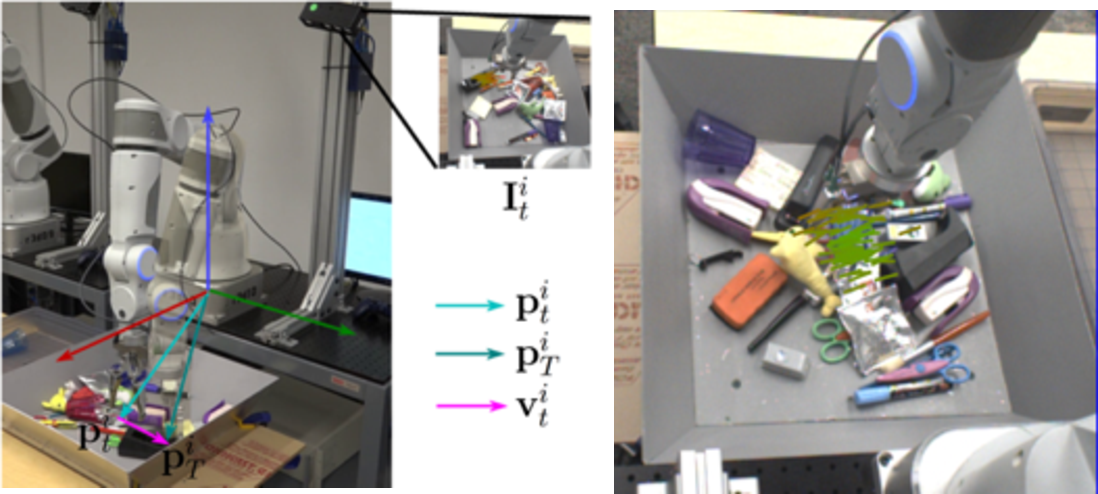
\includegraphics[width=\linewidth]{figure/chapter2/Levine_grasp}
\caption[Colors indicate their probabilities of success: green is 1.0 and red is 0.0]{Colors indicate their probabilities of success: green is 1.0 and red is 0.0\cite{Levine2017}.}
\label{fig:Levine}
\end{figure}
